\documentclass[a4paper]{article}
%\documentclass[letterpaper, 12pt]{CSUniSchoolLabReport}
\usepackage{tikz}
\usetikzlibrary{decorations}
\usetikzlibrary{decorations.pathmorphing}
\usepackage{apacite}
%\usepackage[margin=1in]{geometry} 
% \usepackage{ctex}
\usepackage{tabularx}
%\usepackage{lipsum}
%\usepackage{enumerate}
%\usepackage{amsfonts}
%\usepackage{multirow}
%\usepackage{graphicx}
\usepackage{siunitx}
\usepackage{amsmath}
\usepackage{rotating}
%\usepackage{fbox}
%\usepackage{framed}
%\usepackage{tcolorbox}
\usepackage{colortbl}
\newcommand{\grayrow}{\rowcolor[gray]{0.925}}
\renewcommand{\arraystretch}{1.4}


\begin{document}


\begin{titlepage}
    \title{\textbf{Investigating how the radius of a simple pendulum affect its time period. \\ \small Physics HL Lab Report 5}}
    \author{Eric Zhou}
    \date{\today}
    \maketitle
    %\tableofcontents
\end{titlepage}

\section{Introduction and background knowledge}

Simple pendulum is a phenomenon that has been discovered by humans for a long time. Its periodic behaviour made it an ideal tool for timekeeping long before modern physics has been invented. In physics, the simple pendulum is a great instance to illustrate how physics estabilishes models to interprete real-world phenomenons. 

The period, which is the time taken for the pendulum to do one complete oscillation, varys according to several factors. The effect of the length of string (or rod, depending on the context) is the main focus of this experiment.

\textbf{Research question: What is the relationship between the length of the string and the period of simple pendulum?}
%\section{Background knowledge}
\section{Hypothesis and reasoning}

\begin{figure}[ht]
    \centering
    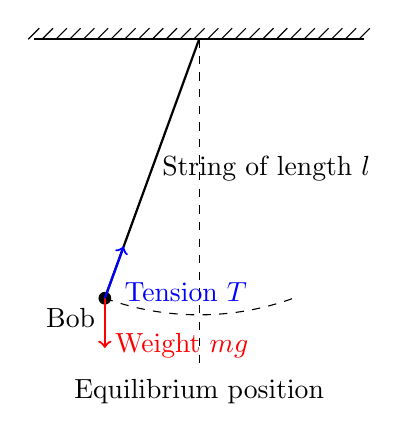
\begin{tikzpicture}[scale = 0.7]

        \def\LBOB{(-1.7101, -4.6984)} % 250 deg
        \def\RBOB{( 1.7101, -4.6984)} % 290 deg
    
        \draw[thick] (0,0) -- \LBOB node[midway,right] {String of length $l$};
    
        \filldraw[black] \LBOB circle (3pt) node[below left] {Bob};
        \draw[dashed] \LBOB arc[start angle = 250, end angle = 290, radius = 5cm];
        \draw[dashed] (0,0) -- (0,-6) node[below] {Equilibrium position};
    
        % Draw the forces
        \draw[->, red, thick] \LBOB -- (-1.7101, -5.6) node[midway, below right] {Weight $mg$};
        \draw[->, blue, thick] \LBOB -- (-1.368, -3.759) node[midway, below right] {Tension $T$};
    
        \foreach \x in {-3.0, -2.75, -2.5, -2.25, -2.0, -1.75, -1.5, -1.25, -1.0, -0.75, -0.5, -0.25, 0.0, 0.25, 0.5, 0.75, 1.0, 1.25, 1.5, 1.75, 2.0, 2.25, 2.5, 2.75, 3.0} 
        \draw[xshift = \x cm] (0.1, 0.2) -- (-0.1, 0);
        
        \draw[thick] (-3,0) -- (3,0) ;
    
        %\filldraw[black] (5, -3) circle (3pt) node[below left]{Bob};
        %\draw[->, blue, thick] (5, -3) -- (5.684, -1.12) node[midway, below right] {Tension $T$};
        %\draw[->, red, thick] (5, -3) -- (5, -5) node[midway, below right] {Weight $mg$};
        %\draw[dashed] (5, -3) -- (5, -1);
    
    \end{tikzpicture}
    \caption{Model of a simple pendulum}
    \label{figp}
\end{figure}

As is shown in Figure \ref{figp}, the bob in a simple pendulum system is subject to two forces: the gravitational force (weight) and the tension from the string. The path of motion is a circle, and therefore the velocity vector must be tangent to the path and perpendicular to the tension all the time. 

When the string is at angle $\theta$ from equilibrium position, we may decomposite the gravitational force into two forces: one at the opposite direction to tension $T$, the other perpendicular to that. It can be noticed that the latter part equals to $mg\sin\theta$. Hence the tangential acceleration can be found by $$a = {mg\sin\theta\over m} = g\sin\theta$$.

It is also worth noticing that the arclength of the bob from equilibrium can be given by $$x = l\theta$$ where $l$ is the length of the string. When $\theta$ is small we have $$\theta \sim \sin \theta \sim \tan \theta$$

Therefore it holds that

$$a \approx g\theta = -{g\over l} x $$

(The negative sign comes from different direction of $a$ and $x$)

Which means that it is valid to say

$$a \propto x$$

showing simple harmonic motion property of the simple pendulum.

According to simple pendulum equations 

$$a = -\omega^2 x$$

$$T = {2\pi \over \omega}$$

We can find that 

$$T = {2\pi\over \sqrt{-a\over x}} = 2\pi\sqrt{l\over g}$$

To make the euqation linear, we can square the both side

$$T^2 = {4\pi^2\over g}l$$

This equation shows a linear relationship between $T^2$ and $l$, which leads to our hypothesis: \textbf{$T$ increases as $l$ gets larger. $T^2$ is directly proportional to $l$.}

\section{Experiment design}

\subsection{Variables}

\begin{itemize}
    \item Independent variable: the length of the string $l$. ($10, 20, 30, 40, 50 \SI{}{cm}$)
    \item Dependent variable: the time period $T$ for the pendulum.
    \item Controlled variables: The size, mass, material of the bob. Initial angle from equilibrium position, etc. They are listed in Table \ref{tab.ctrlvar}.
\end{itemize}

\begin{table}[ht]
    \centering
    \caption{Controlled Variables}
    \label{tab.ctrlvar}
    \vspace{0.2cm}
    \begin{tabularx}{\textwidth}{p{2.0cm} p{1.5cm} X X} % Adjust the width of the second column
        \hline \hline
        \textbf{Variable} & \textbf{Value} & \textbf{Reason to control} & \textbf{Method to control} \\ \hline
        \grayrow The diameter of the bob $d$ & $\SI{2.2}{cm}$ & Make air resistance consistent in different trials & Use the same bob \\ 
        The mass of the bob $m$ & about $\SI{5}{g}$ & Avoid the effect of mass change & Use the same bob \\ 
        \grayrow Initial angle $\theta_i$ & about $20^\circ$ & Make sure the pendulum is equally like SHM & Use a protractor to control the angle. \\ \hline
    \end{tabularx}
\end{table}

\subsection{Materials}

\begin{itemize}
    \item[*] $1 \times$ Iron stand (taller than $\SI{55}{cm}$).
    \item[*] $1 \times$ Electric force gauge (that can display force - time graph on the laptop connected to it).
    \item[*] $1 \times$ Pendulum (contains a string longer than $\SI{50}{cm}$ and a bob attached to it).
    \item[*] $1 \times$ Meter rule.
    \item[*] $1 \times$ Protractor.
\end{itemize}

\subsection{Setup diagram}

As is shown in Figure \ref{fig.setup}, the force gauge is fixed on the top of the iron stand, and the pendulum is attached to the force gauge.

\begin{figure}[ht]
    \centering
    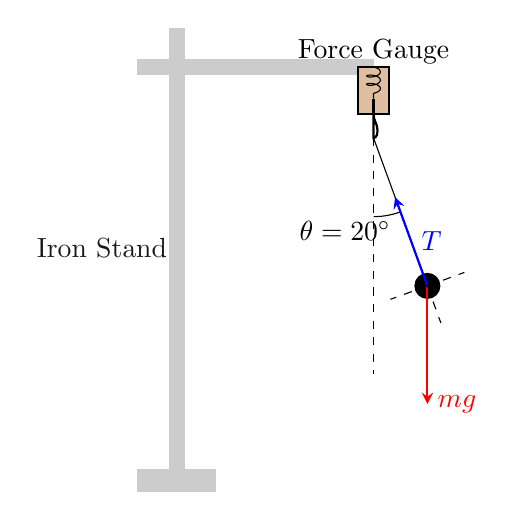
\begin{tikzpicture}[>=stealth]
        % Iron Stand
        \fill[gray!40] (0,0) rectangle (1,-0.3); % Base
        \fill[gray!40] (0.4,0) rectangle (0.6,5.6) node [midway, left, black!90] {Iron Stand}; % Vertical pillar
        \fill[gray!40] (0,5) rectangle (3,5.2); % SHORTENED Horizontal beam (changed from 4 to 3)
    
        % force gauge (adjusted positions for shortened beam)
        \fill[brown!50] (2.8,4.5) rectangle (3.2,5.1); % Casing position adjusted
        \draw[thick] (2.8,4.5) -- (2.8,5.1) -- (3.2,5.1) -- (3.2,4.5) -- cycle;
        
        % Spring mechanism (x-position changed from 4 to 3)
        \draw[decoration={coil,aspect=0.4,segment length=3pt},decorate] (3,5.1) -- (3,4.7);
        \draw[thick] (3,4.7) -- (3,4.5); % Hook stem
        
        % Hook (x-position changed from 4 to 3)
        \draw[thick] (3,4.5) to[out=-90,in=90] (3.05,4.3) to[out=-90,in=0] (3,4.2) -- cycle;
    
        % Pendulum (anchor point changed from 4 to 3)
        \draw (3,4.2) -- ++(-70: 2) coordinate (bob) node[circle,fill=black,minimum size=6pt] {}; % String and bob
        \draw[dashed] (3,4.2) -- (3,1.2); % Equilibrium position
        \draw (3,4.2) ++(0,-1) arc (270:290:1) node[below left] {$\theta = 20^\circ$}; % Angle mark
    
        % Force vectors (anchor point changed from 4 to 3)
        \draw[->,red,thick] (bob) -- ++(0,-1.5) node[right] {$mg$}; % Weight
        \draw[->,blue,thick] (bob) -- ++(110:1.2) node[midway, right] {$T$}; % Tension
        \draw[dashed] (bob) -- ++(20: 0.5);
        \draw[dashed] (bob) -- ++(20: -0.5);
        \draw[dashed] (bob) -- ++(110: -0.5);
     
        % Labels
        \node at (3,5.3) {Force Gauge}; % Position adjusted
    \end{tikzpicture}
    \caption{Setup diagram}
    \label{fig.setup}
\end{figure}

\subsection{Procedure}

\begin{enumerate}
    \item Attach the string to the hook of the force gauge. Use the meter rule to ensure that the length below the hook is $l = \SI{10}{cm}$.
    \item Lift the bob of the pendulum. Make sure the string remains straight. Use the protractor to make sure its angle to vertical is approximately $20^\circ$.
    \item Freely release the bob from stationary. Record the diagram shown on the laptop.
    \item Find a suitable range. Take down the beginning time, ending time and number of crests in the range. 
    \item Repeat steps 2-4 four times to get four additional trials.
    \item Repeat steps 1-5 with $l = 20, 30, 40, 50 \SI{}{cm}$.
\end{enumerate}

\section{Results}

\subsection{Raw data}

As is mentioned in Procedure part, the string length, number of time span, start time and end time are recorded in the experiment. Five groups of experiment were done with five trials each group. 

\begin{table}[!ht]
    \centering
    \caption{Raw Data (full table in appendix)}
    \label{tab.rawd}
    \begin{tabularx}{\textwidth}{p{1cm} X p{1cm} X X X}
    \hline
        Group No. & String length $l(\SI{}{cm})$ & Trial No. & Start time $t_0$ & End time $t_1$ & Number of periods $n$ \\ \hline
        \grayrow 1 & 10 & 1 & 15.1 & 28.9 & 40  \\ %\hline
        1 & 10 & 2 & 6.4 & 19.8 & 40  \\ %\hline
        \grayrow 1 & 10 & 3 & 9.8 & 23.3 & 40  \\ %\hline
        1 & 10 & 4 & 8.6 & 22.2 & 40  \\ %\hline
        \grayrow 1 & 10 & 5 & 11.3 & 24.8 & 40  \\ %\hline
        2 & 20 & 1 & 27.7 & 46.8 & 40  \\ %\hline
        \grayrow$\cdots$ & $\cdots$ & $\cdots$ & $\cdots$ & $\cdots$ & $\cdots$ \\ %\hline
        5 & 50 & 5 & 13.9 & 27.8 & 19  \\ \hline
    \end{tabularx}
\end{table}

\subsection{Processed data}

The processed data can be seen in Table \ref{tab.proc}. Period for the simple pendulum, its square, and their errors are calculated. The method of calculation is illustrated in Sample Processing part.

\begin{table}[!ht]
    \centering
    \caption{Processed data}
    \label{tab.proc}
    \vspace{0.2cm}
    \begin{tabularx}{0.9\textwidth}{XXXXXX}
    \hline
        Group & $T(\SI{}{s})$ & $\Delta T(\SI{}{s})$ & $\%\Delta T(\SI{}{s})$ & $T^2(\SI{}{s^2})$ & $\Delta T^2(\SI{}{s^2})$   \\ \hline
        \grayrow 1 & 0.678  & $\pm$ 0.2 & $\pm$ 1.45\% & 0.46  & $\pm$ 0.013   \\ %\hline
        2 & 0.953  & $\pm$ 0.25 & $\pm$ 1.31\% & 0.91  & $\pm$ 0.024   \\ %\hline
        \grayrow 3 & 1.141  & $\pm$ 0.15 & $\pm$ 0.88\% & 1.30  & $\pm$ 0.023   \\ %\hline
        4 & 1.304  & $\pm$ 0.05 & $\pm$ 0.38\% & 1.70  & $\pm$ 0.013   \\ %\hline
        \grayrow 5 & 1.446  & $\pm$ 0.2 & $\pm$ 1.48\% & 2.09  & $\pm$ 0.062   \\ \hline
    \end{tabularx}
\end{table}

$T-L$ graph and $T^2-L$ graph are plotted, as is shown in Figure \ref{fig.proc}. Linear regression is also done on $T^2-L$ graph. 

\begin{figure}[ht]
    \centering
    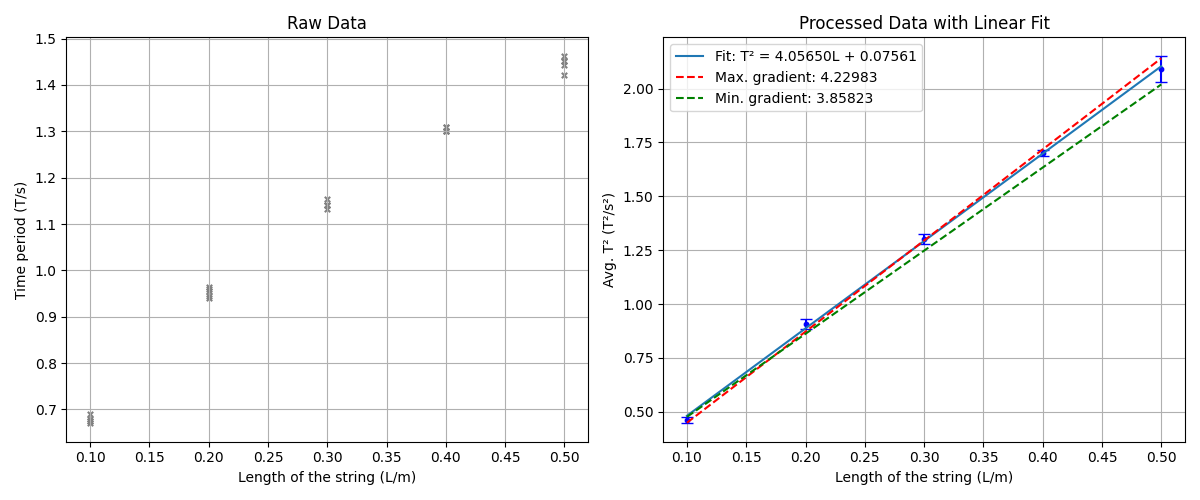
\includegraphics[width = \textwidth]{figure/Figure_1.png}
    \caption{$T-L$ graph and $T^2 - L$ graph}
    \label{fig.proc}
\end{figure}

\subsection{Sample processing}

Take processing of group 1 data as an example, the pendulum time period can be given by $t_1-t_0\over \frac{1}{2} n$ (since in one complete oscillation, the force gauge reaches the crest twice)

$$T_a = {{t_1}_a - {t_0}_a \over \frac{1}{2}n} = {28.90 \SI{}{s} - 15.10 \SI{}{s} \over 20} = 0.69 \SI{}{s}$$

$$T_b = {{t_1}_b - {t_0}_b \over \frac{1}{2}n} ={ 19.80 \SI{}{s} - 6.40 \SI{}{s} \over 20} = 0.67 \SI{}{s}$$

$$\cdots$$

$$T = {t_a + t_b + t_c + t_d + t_e \over 5} \approx 0.68 \SI{}{s}$$

And the error is calculated according to error propangation,

$$\pm 0.5 \Delta T = \pm {\max\{T\} - \min\{T\} \over 2} = \pm 0.01 \SI{}{s}$$

$$\%\Delta T = \pm {\Delta T \over T} \times 100\% = \pm 1.47\%$$

$$T^2 = (0.68 \SI{}{s})^2 \approx 0.46 \SI{}{s^2}$$

$$\Delta T^2 = 2\%\Delta T \times T^2 = \pm 0.013 \SI{}{s^2}$$

\section{Discussion and conclusion}

The diagram shows strong correlation of $T^2$ and $L$. The best fit line of $T^2 - L$ has 

\begin{itemize}
    \item a gradent of $4.056 \SI{}{s^2m^{-1}}$.
    \item a y-intercept of $7.561\times 10^{-2} \SI{}{s^2}$.
\end{itemize}

As is mentioned in processed data section, the graph is expected to be a straight line passing through the origin. The diagram show a graph with relatively small error, supporting the initial hypothesis. 

The y-intercept is expected to be zero, but $7.561\times 10^{-2}$ is found. This is a pretty small amount and it might have resulted from the random error due to limiting accuracy of the device or the sampling frequency has been set too low.

The gradient is expected to be $4\pi^2 \over g$, where $g$ is the gravitational acceleration near sea level $g\approx \SI{9.81}{ms^{-2}}$. The theoratical value of the gradient should be $4.024$, which means there is an $0.7\%$ error. This low error shows high accuracy and precison of this experiment, considering the pendulum is not exactly SHM.

Error bars are relatively small, indicating high precison and low random error. 

% Min fit line, Max fit line. 

\section{Evaluation}

The experiment was conducted successfully, gathering sufficient data and supporting our hypothesis. However, there is still room for improvement. 

\begin{itemize}
    \item \textbf{Defect in SHM pendulum model} Our hypothesis is based on $\sin\theta\approx\theta$. However, the $\theta$ is not very small in the experiment, indicating the bob is not doing perfect SHM. A better model, which may involve ODE (Ordinary Differential Equation), can provide a better hypothesis.
    \item \textbf{Air resistance and friction} We ignore the air resistance and friction between the string and hook in the experiment. Those force may slow down the pendulum and cause its period to change. It is not practical to completely eliminate those effects, but using a heavier bob and smoother string can reduce its effect on the result. 
    \item \textbf{Unfixed apparatus} Some viberation was noticed during the experiment. Additionaly, the string tied to the hook did not remain on the same position either. This may cause the pivot point that is assumed to be fixed to change its position during the experiment, making data inaccurate. Using a steadier iron stand and a smaller hook can fix this issue. 
    \item \textbf{Not on the same surface} When releasing the bob, the hand may exert a force that deviate the bob's motion from the horizontal plane it was supposed to be in. This disturbance may make the motion similar to a cone pendulum. To fix that, we may use an iron bob and electromagnet to lift and release the bob.
\end{itemize}

\clearpage

%\appendix

%\section*{Appendix}

\begin{sidewaystable}[!ht]
    \centering
    \caption{Full data}
    \label{tab.full}
    \begin{tabularx}{\textwidth}{ X X X X X X X X X X X X X }
    %\vspace{0.2cm}
    %\begin{tabular}{ llllllllll }
    \hline
        Group & $l(\SI{}{cm})$ & Trial &  $t_0(\SI{}{s})$ &  $t_1(\SI{}{s})$ & $n$ & $\Delta t(\SI{}{s})$ &  $T(\SI{}{s})$ & $\bar{T}(\SI{}{s})$ & $\Delta T(\SI{}{s})$ & $\%\Delta T(\SI{}{s})$ & $T^2(\SI{}{s^2})$ & $\Delta T^2(\SI{}{s^2})$  \\ \hline
        \grayrow 1 & 10 & 1 & 15.1 & 28.9 & 40 & 13.8 & 0.69  & 0.68  & 0.20  & 1.45\% & 0.46  & 0.01   \\ %\hline
        1 & 10 & 2 & 6.4 & 19.8 & 40 & 13.4 & 0.67  & ~ & ~ & ~ & ~ &   \\ %\hline
        \grayrow 1 & 10 & 3 & 9.8 & 23.3 & 40 & 13.5 & 0.68  & ~ & ~ & ~ & ~ &   \\ %\hline
        1 & 10 & 4 & 8.6 & 22.2 & 40 & 13.6 & 0.68  & ~ & ~ & ~ & ~ &   \\ %\hline
        \grayrow 1 & 10 & 5 & 11.3 & 24.8 & 40 & 13.5 & 0.68  & ~ & ~ & ~ & ~ &   \\ %\hline
        2 & 20 & 1 & 27.7 & 46.8 & 40 & 19.1 & 0.96  & 0.95  & 0.25  & 1.31\% & 0.91  & 0.02   \\ %\hline
        \grayrow 2 & 20 & 2 & 4.5 & 23.3 & 40 & 18.8 & 0.94  & ~ & ~ & ~ & ~ &   \\ %\hline
        2 & 20 & 3 & 8.6 & 27.8 & 40 & 19.2 & 0.96  & ~ & ~ & ~ & ~ &   \\ %\hline
        \grayrow 2 & 20 & 4 & 5 & 24.3 & 40 & 19.3 & 0.97  & ~ & ~ & ~ & ~ &   \\ %\hline
        2 & 20 & 5 & 6.6 & 25.5 & 40 & 18.9 & 0.95  & ~ & ~ & ~ & ~ &   \\ %\hline
        \grayrow 3 & 30 & 1 & 25.4 & 42.5 & 30 & 17.1 & 1.14  & 1.14  & 0.15  & 0.88\% & 1.30  & 0.02   \\ %\hline
        3 & 30 & 2 & 41.4 & 58.7 & 30 & 17.3 & 1.15  & ~ & ~ & ~ & ~ &   \\ %\hline
        \grayrow 3 & 30 & 3 & 8.9 & 25.9 & 30 & 17 & 1.13  & ~ & ~ & ~ & ~ &   \\ %\hline
        3 & 30 & 4 & 33 & 50.1 & 30 & 17.1 & 1.14  & ~ & ~ & ~ & ~ &   \\ %\hline
        \grayrow 3 & 30 & 5 & 8.9 & 26 & 30 & 17.1 & 1.14  & ~ & ~ & ~ & ~ &   \\ %\hline
        4 & 40 & 1 & 13 & 26 & 20 & 13 & 1.30  & 1.30  & 0.05  & 0.38\% & 1.70  & 0.01   \\ %\hline
        \grayrow 4 & 40 & 2 & 15.9 & 29 & 20 & 13.1 & 1.31  & ~ & ~ & ~ & ~ &   \\ %\hline
        4 & 40 & 3 & 11.2 & 24.3 & 20 & 13.1 & 1.31  & ~ & ~ & ~ & ~ &   \\ %\hline
        \grayrow 4 & 40 & 4 & 6.3 & 19.3 & 20 & 13 & 1.30  & ~ & ~ & ~ & ~ &   \\ %\hline
        4 & 40 & 5 & 5.4 & 18.4 & 20 & 13 & 1.30  & ~ & ~ & ~ & ~ &   \\ %\hline
        \grayrow 5 & 50 & 1 & 3.8 & 17.3 & 19 & 13.5 & 1.42  & 1.45  & 0.20  & 1.48\% & 2.09  & 0.06   \\ %\hline
        5 & 50 & 2 & 59.4 & 73.2 & 19 & 13.8 & 1.45  & ~ & ~ & ~ & ~ &   \\ %\hline
        \grayrow 5 & 50 & 3 & 28.8 & 42.5 & 19 & 13.7 & 1.44  & ~ & ~ & ~ & ~ &   \\ %\hline
        5 & 50 & 4 & 18.4 & 32.2 & 19 & 13.8 & 1.45  & ~ & ~ & ~ & ~ &   \\ \hline
    \end{tabularx}
\end{sidewaystable}

\end{document}